% flashcards-title: Number line stretch from 30 to 40 with a dot on 38
% flashcards-desc: The stretch of a number line from 30 to 40 with a mark at every whole number. The end marks are labeled 30 and 40, a dashed vertical guide marks the halfway value labeled 35, and a round dot labeled 38 sits on the mark two steps left of 40.
\documentclass[tikz]{standalone}
\usetikzlibrary{arrows.meta,patterns}

\definecolor{qraNavy}{HTML}{17324D}
\definecolor{qraBlue}{HTML}{2B6CB0}
\definecolor{qraGold}{HTML}{B7791F}
\definecolor{qraPale}{HTML}{EAF2F8}
\definecolor{qraGray}{HTML}{5C6773}

\tikzset{
  qra axis/.style={draw=qraNavy, line width=1.2pt},
  qra tick/.style={draw=qraNavy, line width=1pt},
  qra guide/.style={draw=qraGray, densely dashed, line width=0.8pt},
  qra counter/.style={circle, draw=qraNavy, fill=qraPale, line width=0.9pt, minimum size=7mm, inner sep=0pt},
  qra label/.style={font=\sffamily\bfseries, text=qraNavy},
  qra small label/.style={font=\sffamily, text=qraNavy},
}

\begin{document}
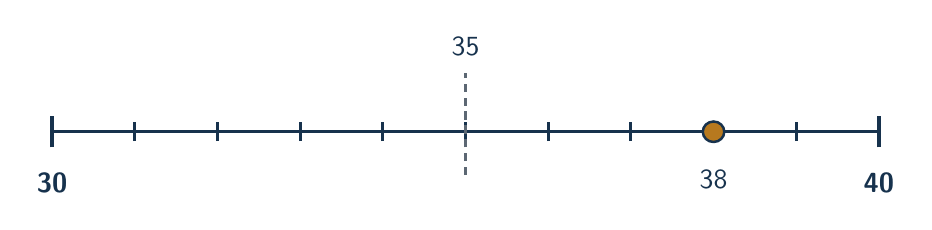
\begin{tikzpicture}[x=1.05cm]
  % Line segment from 30 (x=0) to 40 (x=10)
  \draw[qra axis] (0,0) -- (10,0);

  % Unit ticks; taller ticks at the two tens
  \foreach \n in {1,...,9} {
    \draw[qra tick] (\n,-0.12) -- (\n,0.12);
  }
  \draw[qra tick, line width=1.3pt] (0,-0.2) -- (0,0.2);
  \draw[qra tick, line width=1.3pt] (10,-0.2) -- (10,0.2);
  \node[qra label, below=2.5mm] at (0,-0.15) {30};
  \node[qra label, below=2.5mm] at (10,-0.15) {40};

  % Halfway value: dashed guide and label
  \draw[qra guide] (5,-0.55) -- (5,0.75);
  \node[qra small label, above=1mm] at (5,0.75) {35};

  % Dot on 38 with its numeral beneath
  \filldraw[fill=qraGold, draw=qraNavy, line width=0.9pt] (8,0) circle (0.13);
  \node[qra small label, below=2.5mm] at (8,-0.12) {38};
\end{tikzpicture}
\end{document}
